% Preamble
\documentclass[a4paper,12pt]{article}

\usepackage[osf]{mathpazo} % palatino
\usepackage{ms}            % load the template
\usepackage[round]{natbib} % author-year citations
\usepackage{graphicx}
\usepackage{parskip} 
\usepackage{enumerate} 
%\usepackage[nomarkers, nolists]{endfloat}  % To push floats to the end   
\pagenumbering{arabic}    

% Title page information

\title{A cautionary note on the use of Ornstein Uhlenbeck and other models in macroevolutionary studies}
\author{
  Natalie Cooper$^{1,2,*,\dag}$, Gavin H. Thomas$^{3,\dag}$, Chris Venditti$^{4}$\\ Andrew Meade$^{4}$ and Rob P. Freckleton$^{3}$\\
}
\date{}
\affiliation{\noindent{\footnotesize
  
  $^1$ School of Natural Sciences, Trinity College Dublin, Dublin 2, Ireland.\\ 
  $^2$ Trinity Centre for Biodiversity Research, Trinity College Dublin, Dublin 2, Ireland.\\
  $^3$ Department of Animal and Plant Sciences, University of Sheffield, Sheffield S10 2TN, UK.\\
  $^4$ School of Biological Sciences, University of Reading, Reading, Berkshire, RG6 6BX, UK.\\
  $^*$ Corresponding author: ncooper@tcd.ie; Zoology Building, Trinity College Dublin, Dublin 2, Ireland. 
       Fax: +353 1 677 8094; Tel: +353 1 896 1926.\\
  $^\dag$These authors contributed equally.
}}

\vfill
%\paragraph{Word-count:} X words

\runninghead{A cautionary note on macroevolutionary models}
\keywords{Bayesian method - comparative methods - delta - kappa - lambda - OU - phylogeny - stabilizing selection - selection} %meant to be after abstract

% End of preamble

\begin{document}
\modulolinenumbers[1]   % Line numbering on every line

\mstitlepage
\parindent = 1.5em
\addtolength{\parskip}{.3em}

\section{Abstract 100-200}
  %Phylogenetic comparative methods are increasingly used to give new insight into variation, causes and consequences of trait variation among species. The foundation of these methods is a suite of models that attempt to capture evolutionary patterns by extending the Brownian constant variance model. However, the parameters of these models have been hypothesised to be biased and only asymptotically behave in a statistically predictable way as datasets become large. This does not seem to be widely appreciated. We show that a commonly used model in evolutionary biology (the Ornstein-Uhlenbeck model) is biased over a wide range of conditions. Many studies fitting this model use datasets that are small and prone to substantial biases. Our results suggest that simulating fitted models and comparing with empirical results is critical when fitting OU and other extensions of the Brownian model. 

\newpage
\raggedright
\doublespacing
\setlength{\parindent}{1cm}

\section{Introduction}
\label{section:introduction} 

  Phylogenetic comparative methods are powerful tools for identifying patterns in the evolution of species traits, and for potentially inferring the evolutionary processes that underlie them \citep[e.g.,][]{freckleton2009seven,Nunn:2011aa,o2012evolutionary,pennell2013integrative}. 
  These approaches have been used, for example, to infer potential rates of species responses to climate change \citep{Quintero:2013aa}, test the role of ecological niche as a driver of morphological evolution \citep{pienaar2013macroevolution}, and test for constraints in adaptive radiations \citep{blackburn2013adaptive}. 
  %Unfortunately, although widely used, the properties of some phylogenetic comparative methods are poorly understood leading to the potential for inappropriate use and misinterpretation of results. 

  Most model-based methods for characterizing trait evolution are based on the Brownian constant variance model \citep[for exceptions see][]{price1997correlated,harvey2000comparative,freckleton2006detecting}. 
  The Brownian model, first applied in a phylogenetic context by \citet{cavalli1967} and to across-species data by \citet{felsenstein1973maximum}, is a simple model of trait evolution in which trait variance accrues as a linear function of time, and makes the prediction that traits of closely-related species are more similar than those of distantly-related ones. 
  The Brownian model has been modified in various ways to account for a suite of ecological and evolutionary processes \citep[e.g.,][]{grafen1989phylogenetic,hansen1997stabilizing,Pagel:1997aa,Pagel:1999aa}. 
  The majority of these involve a transformation of the tree and thereby fitting a model with one or more extra parameters. 
  These modified Brownian models tend to fit better and often have links to process-based interpretations. 

  One of the most commonly used Brownian-like models is the Ornstein Uhlenbeck (OU) model. 
  This is a modification of the Brownian model with an additional parameter $\alpha$ that measures the strength of return towards a theoretical optimum \citep{hansen1997stabilizing}. 
  The OU model was introduced to population genetics by \cite{Lande:1976aa} to model stabilizing selection in which the trait mean was recast as a fitness optimum on an adaptive landscape. 
  The process operating in comparative data is analogous, although clearly is not stabilizing selection, despite being sometimes referred to as such (see Discussion).

  The popularity of the OU model has grown extensively in recent years (Fig. \ref{figure.literature}); over 2500 ecology, evolution and palaeontology papers containing the phrase ``Ornstein Uhlenbeck'' were published between 2012 and 2014 (Google Scholar search 15th March 2015; see Supplementary Material). % Need to add ref to supp mat
  This may partly be because these models are now easy to implement apply via packages in R \citep[e.g. ouch, GEIGER and OUwie;][]{Butler:2004aa,Harmon:2008aa,beaulieu2012ouwie}. 
  Additionally, although the OU model is pattern-based, it has a number of attractive biological interpretations. 
  For example, fit to an OU model is used as evidence for processes such as phylogenetic niche conservatism, convergent evolution and stabilising selection \citep[e.g.,][]{Wiens:2010aa,christin2013anatomical,ingram2013surface}. 
  Unfortunately, although widely used, the properties of the OU model are poorly understood leading to the potential for inappropriate use and misinterpretation of results. 
 
    \begin{figure}[h]
      \centering
      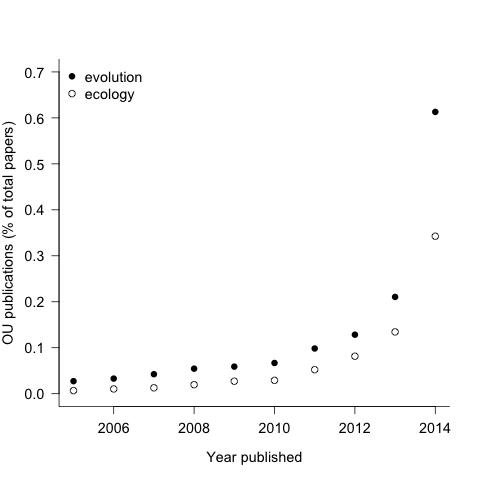
\includegraphics[width=10cm, height=10cm, keepaspectratio=true]{Figures/PapersThruTime.png}
      \caption{The number of ecology, evolutionary biology and palaeontology papers published between 2005 and 2014 containing the phrase ``Ornstein-Uhlenbeck'', as a proportion of the total number of ecology, evolutionary biology or palaeontology papers published that year. See Supplementary Material for details %linkto supp mat
      }
      \label{figure.literature}
    \end{figure}

  The OU model is most commonly used to model the evolution of a continuous character (Table \ref{table.uses}; Supplementary Material). 
  Multiple models of evolution \citep[e.g., Brownian motion, OU, Early burst etc.;][]{Harmon:2010aa,cooper2010body} are fit to the same continuous character and model selection is then used to determine which model best fits the data.  
  OU models can be fit with one optimal trait value, or multiple different optima \citep{Butler:2004aa,beaulieu2012modeling}. 
  The latter represents evolution under multiple selective regimes, and may be more biologically realistic. 
  OU models with various numbers of optima are often included in the pool of evolutionary models being compared \citep[e.g.,][]{} (Table \ref{table.uses})
  
  OU models are also commonly used to control for phylogeny in correlative analyses (Tables \ref{table.uses}; Supplementary Material).  
  Phylogenetic generalised least squares (PGLS) models incorporate information about the relationships among species into the error term of a generalised least squares model. 
  This error term generally consists of a variance-covariance matrix of the phylogeny, but various transformations are used (e.g., Pagel's $\lambda$; \citealp{Pagel:1997aa}) to improve the fit of the model to the data. 
  The $\alpha$ parameter from an OU model can also be used to transform the tree and the variance-covariance matrix.
  This is rarely interpreted as corresponding to any kind of process, it just improves the fit of the PGLS models \citep[e.g.,][]{blankers2012ecological}. Finally, the OU model is also used to reconstruct ancestral states \citep{martins1999estimation} and to detect clade-wide convergent evolution \citep{ingram2013surface}. 

  The majority of papers use the OU model to model the evolution of a continuous character (Table \ref{table.uses}; Supplementary Material) therefore, we focus on this use of the OU model in our simulations below. 
  The principles here also apply to a range of other macroevolutionary models that can be fit to continuous data and compared using model testing procedures.
  Note that we focus on OU models with a single optimum trait value because these are more commonly used (Table \ref{table.uses}; Supplementary Material) and easier to simulate, but our general conclusions also apply to multiple optima OU models.

    \begin{table}[h]
        \caption{The most common uses of Ornstein Uhlenbeck models in ecology, evolutionary biology and palaeontology papers published between 2005 and 2013. See Supplementary Material for details.}
        \bigskip  
          \begin{tabular}{p{8cm}lc}
            \hline
            Use of OU model & Optima & Number of papers\\
            \hline
            Ancestral state reconstruction & single & 8\\
            & multiple & 2\\
            Convergent evolution & single & 0\\
            & multiple & 2\\
            Model of evolution & single & 31\\
            & multiple & 27\\
            Phylogenetic generalised least squares & single & 35\\
            & multiple & 0\\
            Other & single & 5\\
            & multiple & 5\\
            Total & single &  36\\
            & multiple & 79\\
            \hline
            \label{table.uses}
          \end{tabular}
    \end{table}

  Here we present simulations demonstrating the inherent bias in estimating the $\alpha$ parameter, discuss the intricacies of interpreting OU models biologically, and provide advice for appropriate use of OU models in phylogenetic comparative analyses. We also show that very small amounts of measurement error in data can have profound effects on the performance of models. 
  Many of our findings are applicable to other models of evolution (see Discussion and Supplemental Figs. S6-S11) 
  % Add figure refs here
  , but we focus on the OU model because of the recent increase in publications using the model and because of the under-appreciated ambiguity in the link between pattern and process when interpreting estimates of the $\alpha$ parameter. 
  We are not the first to mention these problems, but we hope by summarising the issues and giving recommendations we can help those less familiar with the technical literature \citep[e.g.,][]{ho2013asymptotic,ho2014intrinsic,boettiger2012your,hansen2012interpreting,ives2010phylogenetic}.

\section{Materials and Methods}
  \subsection{The Ornstein Uhlenbeck (OU) model}
    According to the Brownian model \citep{cavalli1967,felsenstein1973maximum}, a trait X evolves at random at a rate $\sigma$:

      \begin{equation}
        dX(t) = \sigma dW(t)
      \end{equation}
    
    \noindent
    where $W(t)$ is drawn at random from a normal distribution with mean $0$ and variance $\sigma^2$. 
    The model assumes that there is no overall drift in the direction of evolution (hence the expectation of $W(t)$ is zero) and that the rate of evolution is constant. 
    Because the direction of change in trait values at each step is random, Brownian motion is often described as a ``random walk''.
    The model assumes the correlation structure among trait values is proportional to the extent of shared ancestry for pairs of species. 
    This means that close relatives will be more similar in their trait values than more distant relatives. It also means that variance in the trait will increase (linearly) in proportion to time. 
    The model has two parameters, the Brownian rate parameter, $\sigma^2$ and the state of the root at time zero, $X(0)$. 

    The OU model \citep{hansen1997stabilizing,Butler:2004aa} is a random walk where trait values revert back towards some ``optimal'' value with an attraction strength proportional to the parameter $\alpha$. 
    The model has the following form:
  
      \begin{equation}
        dX(t) = - \alpha (X(t) - \mu) + \sigma dW(t)
      \end{equation}
    
    \noindent
    Note that this model has two parameters in addition to those of the Brownian model: $\alpha$ and $\mu$. 
    The parameter $\mu$ is a long-term mean, and it is assumed that species traits evolve around this value. 
    $\alpha$ is the strength of evolutionary force that returns traits back towards the long-term mean if they evolve away from it. 
    $\alpha$ is sometimes referred to as the ``rubber band'' parameter because of the way it pulls traits back towards $\mu$. For more details see the Appendix.
    
    When $\alpha$ is close to zero, evolution is approximately Brownian, then as $\alpha$ gets larger the non-Brownian behaviour of the model starts to become apparent. 
    Eventually, when $\alpha$ is really large, all imprint of history is lost and the trait evolution is essentially a rapid burst at the present.

    $\alpha$ can more easily be interpreted by using it to estimate the ``phylogenetic half-life'' ($t_\frac{1}{2}$) of a trait, i.e., the time it takes for a species entering a new niche to evolve halfway toward its new expected optimum \citep{hansen1997stabilizing}, as follows:

      \begin{equation}
        t_\frac{1}{2} = \frac{ln(2)}{\alpha}
        \label{equation:halflife}
      \end{equation}
    
    \noindent
    This is sometimes referred to as a measure of ``phylogenetic inertia'' but we dislike this term because it means different things to different researchers \citep{Losos:2008aa}.
    If $t_\frac{1}{2}$ is short relative to the branch lengths of the phylogeny, evolution towards the optimum trait value is fast, residual phylogenetic correlations are weak, and there is little influence of the past on trait values \citep{hansen1997stabilizing}. 
  
  \subsection{Known statistical issues with the OU model}
  ???Problems with the OU model and where they are reported in the literature?

    \begin{enumerate}
      \item $\alpha$ is bounded at zero.
      \item blah
      \item measurement errors
    \end{enumerate}

  \subsection{Maximum Likelihood simulations}
  \label{section:sims.methods} 
    We used simulations to explore the statistical properties of $\alpha$. 
    We simulated phylogenies with 25, 50, 100, 150, 200, 500, or 1000 tips under pure birth, constant-rate Birth-Death (extinction fractions of 0.25, 0.5 and 0.75), or temporally varying speciation rate (speciation rate modeled as time from the root raised to the power 0.2, 0.5, 2 and 5) models. 
    We simulated 1000 phylogenies for each combination of tips and models resulting in 56,000 simulated phylogenies in total. 
    Trees were simulated using the R package TESS \cite{hohna2013fast}. 
    We then simulated the evolution of a single trait under a Brownian motion model on each phylogeny using the R package MOTMOT \citep{Thomas:2011aa}. 
    We estimated $\alpha$ and compared the fit of a Brownian model to that of an OU model using a likelihood ratio test with 1 degree of freedom with the \texttt{transformPhylo.ML} function in MOTMOT \citep{Thomas:2011aa}. 
    This procedure mirrors a situation where the OU model  %%% argh

  \subsection{Effects of measurement error}
    Measurement error can strongly effect the results of comparative analyses \cite{silvestro2015} so we also investigated whether adding error to our simulated data influenced estimates of $\alpha$.
    We used the same procedure as above to simulate trait data under a Brownian motion model with known error. 
    Specifically, we simulated trees under a Yule model with 25, 50, 100, 150, 200, 500, or 1000 tips and added branch length of (i) 1\%, (ii) 5\% or (iii) 10\% of the tree height to the tips of the simulated trees. 
    We then simulated data under a Brownian model on each tree. 
    We compared the fit of a Brownian model to that of an OU model using likelihood ratio tests as described above, using the original trees without the addition of extra branch length to the tip edges. 
    Our expectation is that the OU model should fit the data better than the Brownian model but the reason for the better fit would be entirely unrelated to any evolutionary process. 

  \subsection{Other evolutionary models}
    Although our focus is on the OU model we also explored three other commonly used models of trait evolution -- $\kappa$, $\lambda$, and $\delta$ \citep{Pagel:1997aa,Pagel:1999aa} -- fitted using Maximum Likelihood with the same simulated data. 
    These models are designed to test for speciational evolution ($\kappa$), strength of phylogenetic signal ($\lambda$) and accelerating or decelerating evolution ($\delta$). 
    The point of these additional tests is to assess the extent to which parameter behaviors vary across models and the results are reported in the Supplementary Material. 

\section{Results}
  \subsection{Maximum Likelihood simulations}
  \label{section:sims.results}
    
    Figure \ref{figure.profiles} shows some examples of profile likelihoods for $\alpha$ generated on different datasets that were simulated according to a Brownian model. It is clear that the shape of the tree affects the shape of the likelihood profile. Trees with increasing speciation rates from root to tip (i.e., that have a lot of recently evolved species) generate very wide, flat likelihood profiles (Fig. \ref{figure.profiles}A). On the other hand, trees with declining speciation rates from root to tip (Fig. \ref{figure.profiles}B), or generated according to a Yule process (Fig. \ref{figure.profiles}C), yield more strongly peaked profiles. 

%\begin{figure}
 % \centering
  %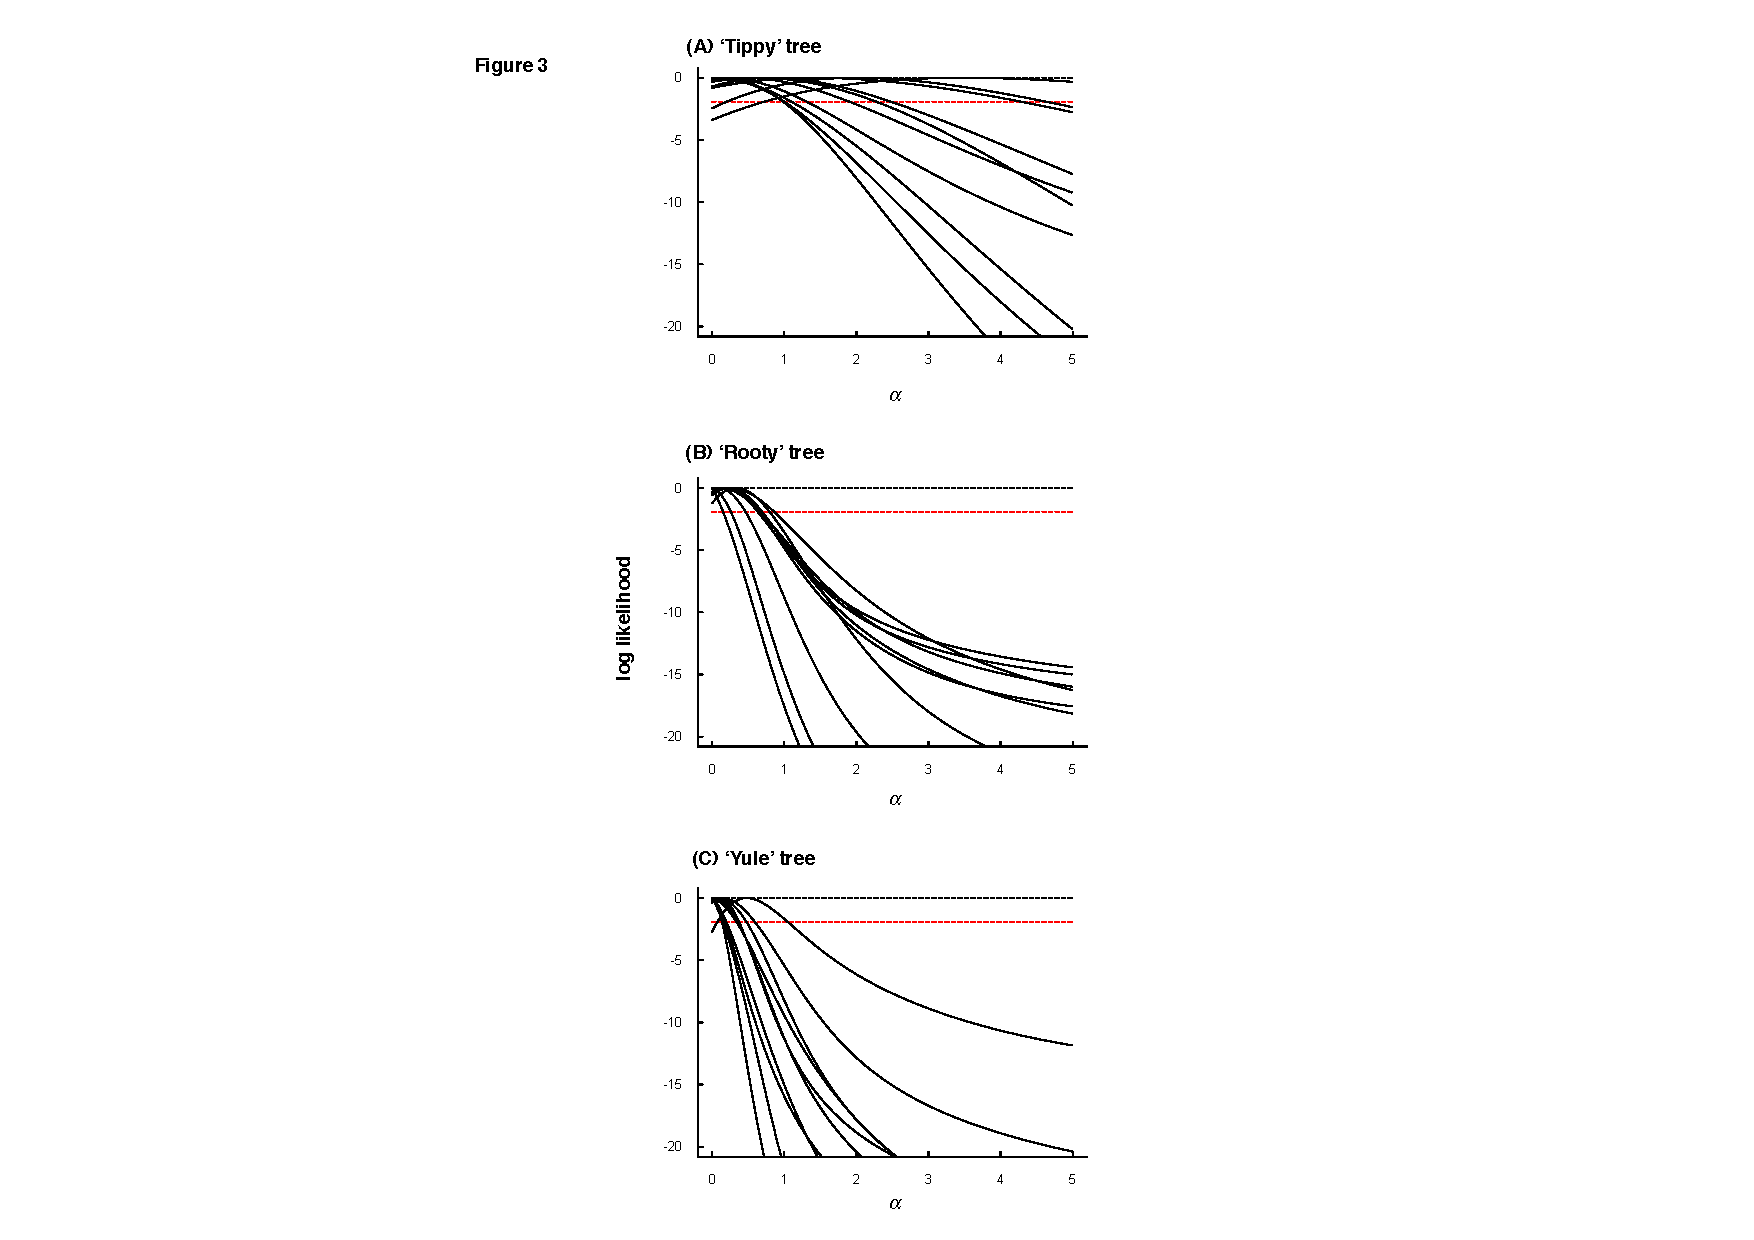
\includegraphics[width=10cm, height=10cm, keepaspectratio=true]{Figures/OU_figure3.pdf}
  %\caption{Examples of profile likelihoods for selected simulated datasets. In all cases the ‘true’ value of alpha is 0.}
%\label{figure.profiles}
%\end{figure}

In all three cases, there are several features worth noting. First, the profiles are asymmetric. There is a hard bound at $\alpha = 0$, and as $\alpha$ becomes large, the rate of decrease in the likelihood slows. This is because, as shown in Figure \ref{figure.traitsim}, as values of $\alpha$ become large, the effects of changing $\alpha$ on model predictions are increasingly small. It is also notable, that the Maximum Likelihood estimates of $\alpha$ are, in most cases, between 0 and 1. In Figure \ref{figure.traitsim} it was noted that in this region of parameter space, the OU model is very difficult to distinguish from Brownian. This, combined with the asymmetric nature of the profile likelihood is suggestive that estimates of $\alpha$ are likely to be biased, and that the asymptotic assumptions of likelihood ratio tests on $\alpha$ are likely to be violated.

The effects of the asymmetric profile likelihoods become clear when calculating Type I error for the OU model based on ML estimates across a range of tree shapes and sizes (Fig. \ref{figure.rejection}; see Supplemental Figs. S2 and S3 for results with alternative priors for the Bayesian analyses). Regardless of tree shape, Type I error rates are unacceptably high when tree size is small (Figs. \ref{figure.rejection}A, \ref{figure.rejection}C and \ref{figure.rejection}E). For some tree shapes (particularly where speciation rates accelerate towards the present), Type I error remains $>0.05$ even for trees with 1000 tips. Bayesian estimation is not subject to bias % check in the log-likelihood statistic and consistently rejects the OU model. However, estimates of α are similar regardless of method.

%\begin{figure}
  %\centering
  %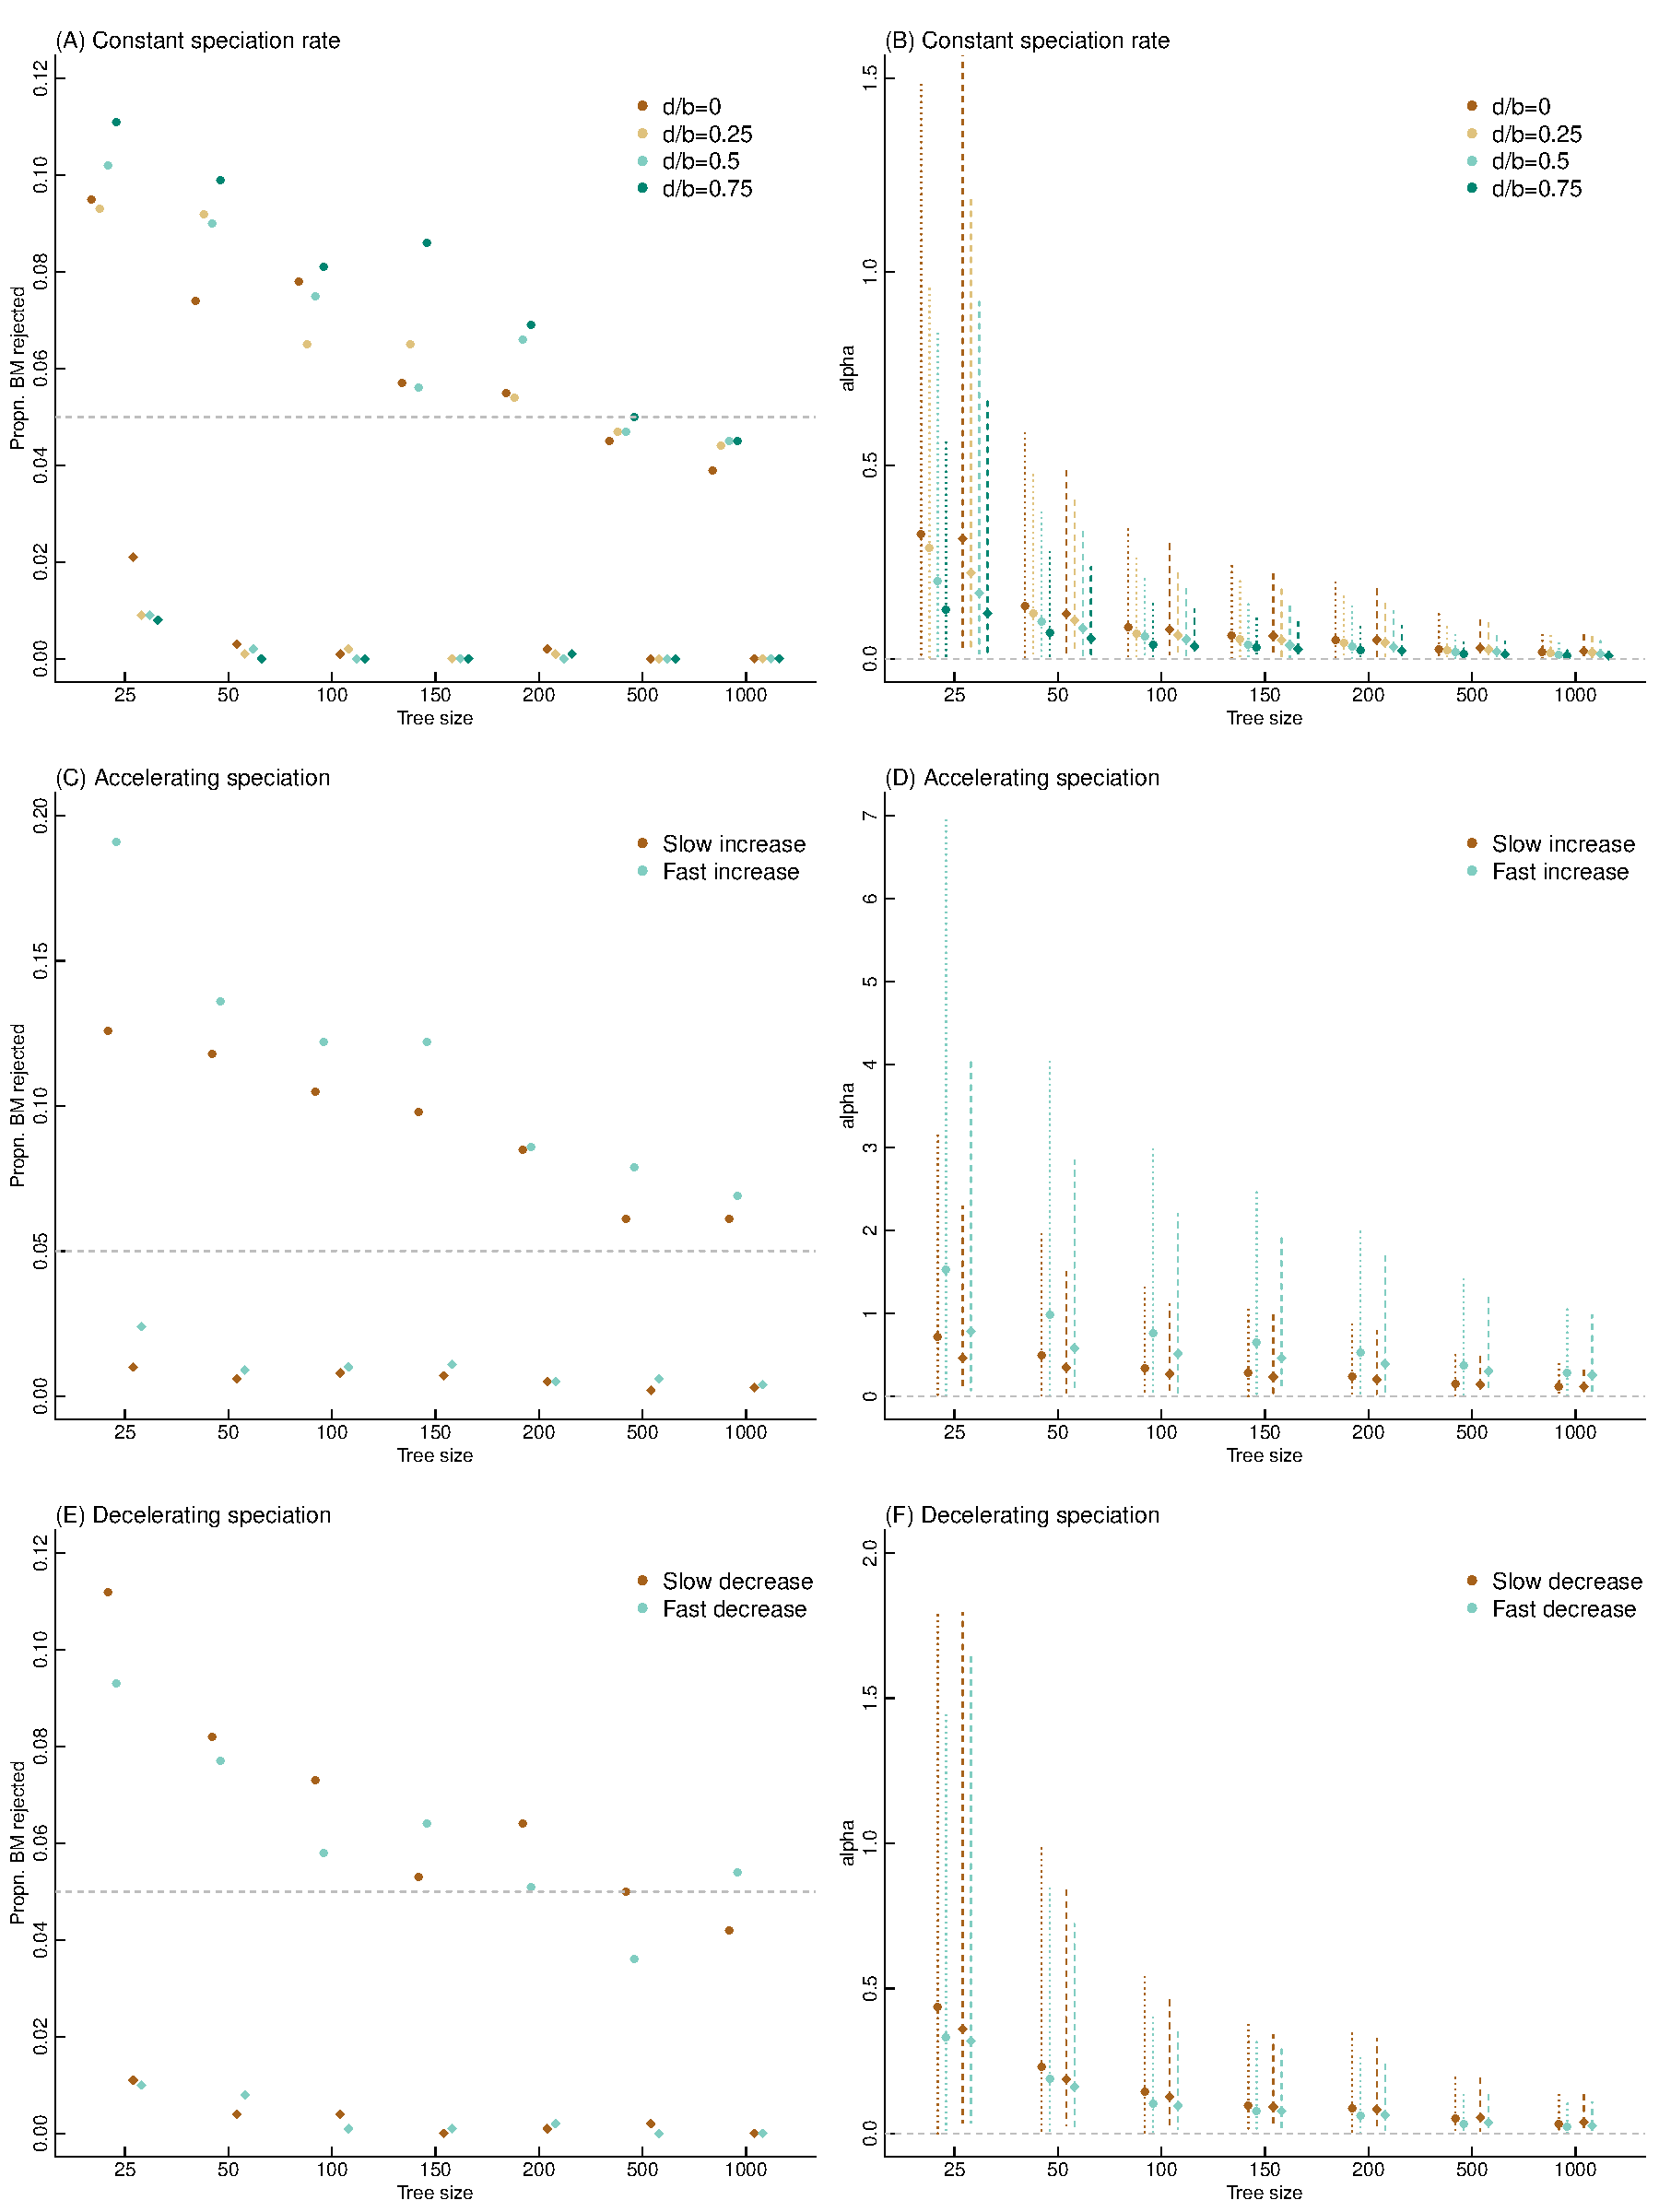
\includegraphics[width=10cm, height=10cm, keepaspectratio=true]{Figures/OU_figure4.pdf}
  %\caption{Rejection rates and estimation of $\alpha$ for different tree sizes and shapes. Rejection rates (a,c,e) for the OU model at multiple tree sizes for models fitted using ML (circles) and Bayesian (diamonds) methods. Estimates of $\alpha$ (b,d,f) based on ML (circles show means and dotted lines show 95\% sampling interval from 1000 trees) and Bayesian (diamonds show means and dotted lines show 95\% sampling interval of the modal value from the posterior distribution from 1000 trees).}
%\label{figure.rejection}
%\end{figure}

%Figure \ref{figure.error} shows the proportion of data sets in which the OU model is favoured over the Brownian model for data simulated under Brownian motion with error (also see Figs. S4 and S5). The expectation is that the OU model should fit better because the branch length transformation partially captures the non-Brownian component (the error). There are two points worth noting. First, the frequency with which the OU model is favoured increases with tree size for both ML and Bayesian estimation (Fig. \ref{figure.error}A). With as little as 5\% error, the OU model becomes extremely difficult to reject, even for trees with just 100 species. This is important for the interpretation of the OU model. We cannot conclude anything about evolutionary process from a single optimum OU model unless error is adequately accounted for. Second, for moderate amounts of error (5-10\%), the ML estimates of $\alpha$ are consistently $>$ 1 (Fig. \ref{figure.error}B). Large values of $\alpha$ are similarly difficult to interpret because they are indicative that the signal of the past has been overwritten. 

%\begin{figure}
 % \centering
  %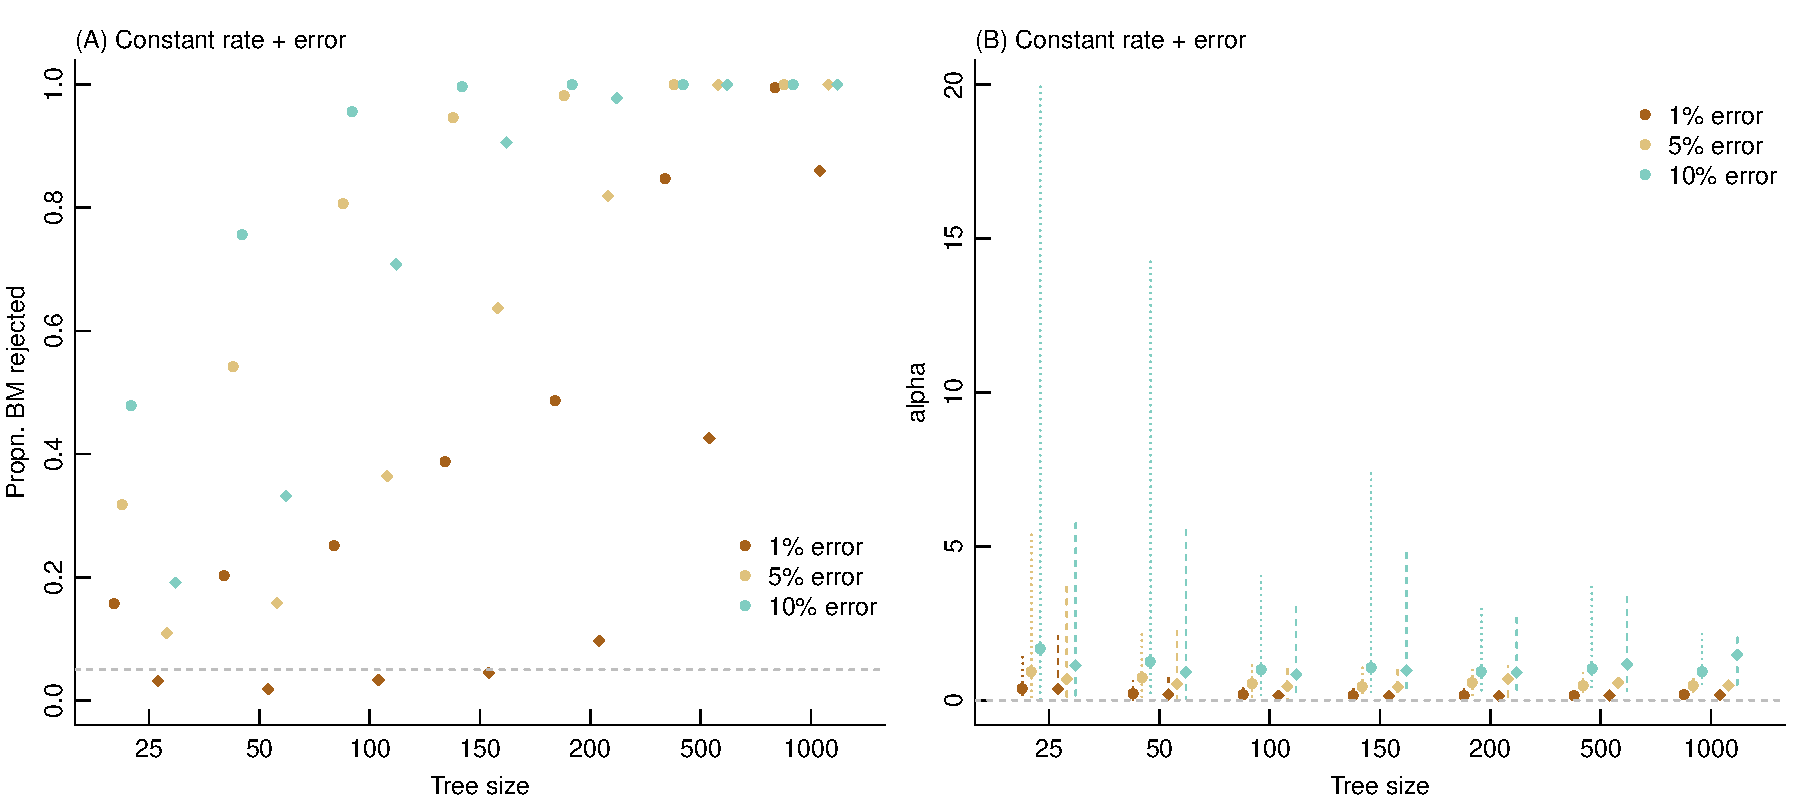
\includegraphics[width=10cm, height=10cm, keepaspectratio=true]{Figures/OU_figure5.pdf}
  %\caption{Rejection of BM with measurement error (a) and estimation of α (b). Symbols follow Figure \ref{figure.rejection}.}
%\label{figure.error}
%\end{figure}

The bias % check
 reported above are not unique to the OU model. The parameter $\delta$, which tests for accelerating or decelerating rates of evolution \citep{Pagel:1997aa,Pagel:1999aa} also suffers from elevated Type I error and is upwardly biased, favoring models that imply temporally increasing evolutionary rates (Supplemental Fig. S8). In contrast, although the speciational model ($\kappa$) has slightly elevated Type I errors, the parameter estimates are unbiased for the majority of tree sizes and shapes (Supplemental Fig. S6). As previously shown (Freckleton et al. 2002), the $\lambda$ model is conservative with low Type I error rates (Supplemental Fig. S7). As with the OU model, the $\delta$ models are all strongly favored over Brownian motion when there is error in the species data (Supplemental Figs. S9-S11). 

\section{Discussion}
\label{section:discussion}

Recommendations

Interpreting results
 - OU is favoured over BM. If alpha is small it's basically BM. What
is alpha? Talk about half lives. add in ives and garland advice on what is big and what is small here?
 - Not stabilising selection
 - Not an issue if you're just mopping up error structure for PGLS (?)
 - If really want to be certain OU over BM you need 200 species
 - Account for measurement error

%Results from \citet{ho2013asymptotic}, indicate that there is the potential for revealing strong biases in $\alpha$ , but the implications for practice (e.g. likelihood of rejection of alternative models) is unexplored other than to note that tree shape may play an influence. 

%The modification of Brownian models to account for non-Brownian processes can be traced back to \citet{grafen1989phylogenetic} who introduced a parameter $\rho$ to account for non-linear scaling of evolutionary changes. $\rho$ is a power transformation of node heights in the phylogeny, and is fitted by maximum likelihood. It is worth noting that Grafen warned explicitly about potential drawbacks with $\rho$. Specifically: (i) the parameter is likely to be biased; (ii) its asymptotic sampling variance is non-zero; and (iii) values of the parameter should be interpreted cautiously. \citet{freckleton2002phylogenetic} showed that $\rho$ was indeed biased as predicted by Grafen (1989). They also showed that another parameter, Pagel’s $\lambda$ \citep{Pagel:1997aa,Pagel:1999aa}, also exhibited biases (but that these were likely to have minimal consequences in analyses using reasonable sample sizes). This strongly suggests that simulations are required to test the properties of such parameters, and that as recommended by \citet{grafen1989phylogenetic} “careless” parameterization of the phylogenetic variance-covariance matrix should be avoided.

Although it is possible to create and implement new models for comparative data that encompass a range of processes, we have to beware that such models are statistically complex and may behave in unexpected ways. Transformations of the variance-covariance matrix in the Brownian model are an attractive and computationally simple way to modify the basic model to include evolutionary processes. But, as first pointed out by \citet{grafen1989phylogenetic}, the statistical consequences of these modifications can include biases and problems with interpretation. The results we have presented here illustrate that such biases can occur under conditions that closely match the size and type of datasets that are commonly used. 

In the case of the OU model, we can make a series of specific recommendations for future analyses:
\begin{enumerate}[(i)]
  \item At least 200 species should be included. The results of the simulations indicate that, in general, analyses based on small datasets are prone to biases that decrease only slowly as the size of the dataset increases.  
  \item Likelihood ratio tests are untrustworthy. We would expect these to be approximate because $\alpha$ is bounded and has a non-linear effect on the expected variances. The simulations indicate that likelihood ratio tests should not be relied upon for analyses with small sample sizes, and that for robust inference and testing, alternatives, such as MCMC, should be considered. 
  \item Simulate fitted models and compare these to your empirical results. A good strategy for data exploration would be to simulate data under BM and fitted OU models to generate distributions of parameters under known values. These can then be compared to results for your dataset \citep[see][for a related approach]{slater2013robust}. This is important because we have shown that the shape of a phylogeny has consequences for parameter biases and hypothesis tests. Any given tree will therefore generate unique parameter estimates. Simulating data under the BM model will generate null distributions \citep[e.g.,][]{boettiger2012your}. Generating data under the fitted OU model will allow an assessment of whether it is possible to retrieve known values, or whether there is evidence of bias. 
  \item Consider plausible alternative hypotheses. The results indicate that a simple parsimonious model can be mistaken for an OU process: namely a BM process in which a small amount of error is added to the data. Small ($<$ 1) values of $\alpha$ are quite compatible with this interpretation of the data. The effects of error become more severe with increasing tree size. 
\end{enumerate}

In terms of the final point, it would be very useful to have estimates of measurement errors for the species’ observations, however the inclusion of species-specific variances has to be done carefully \citep[e.g.,][]{grafen1989phylogenetic}. It would be tempting to create a vector of variances that could be combined with V to create an overall combined variance matrix \citep{o2012evolutionary,Harmon:2010aa}. However, if the variances are large, vary among species or are based on small samples, this can create additional complications for the modeling. This is because the variances will themselves be estimates and subject to error. Treating such variances as error-free can potentially create biases (Freckleton unpub). If the variances are unknown then Pagel’s $\lambda$ \citep{Pagel:1997aa,Pagel:1999aa} can be used to estimate the non-Brownian component of the trait variance. However estimating this parameter simultaneously with estimating $\alpha$ would have to be undertaken carefully as the two transformations have quite similar effects on the predicted variances. 

Our review of the literature revealed that the OU model is frequently described and interpreted as a model of ‘stabilizing selection’. The OU model is attractive because it sets effective bounds in probability on the size of species’ traits, but to use the term ‘stabilizing selection’ is inaccurate and misleading. As formulated by \citet{hansen1997stabilizing}, a niche has a primary optimum that is the mean of individual species optima for that niche. Under this formulation, α can be considered as the strength of the pull towards the primary optima \citep{hansen2012adaptive} but not as an estimate of stabilizing selection in the population genetics sense. 

In terms of interpretation, it is worth pointing out that data will exhibit few signs of the limits to trait values that result from an OU process. This is because according to the OU process traits move back towards the optimum as their values become particularly large or small. Past history is effectively wiped over, as pointed out above, with the consequence that covariances between species become small (Fig. \ref{figure.traitsim}). Indeed, Figure \ref{figure.traitsim} implies that the outcome of the OU process is indistinguishable from an acceleration of the rate of evolution towards the present. This interpretation is particular important for inference of phylogenetic niche conservatism. Although definitions of phylogenetic niche conservatism vary \citep{Losos:2008aa,Losos:2008ab,Wiens:2008aa,crisp2012phylogenetic} one proposed approach is to fit an OU model and take rejection of BM in favour of OU as evidence of constraints on niche evolution \citep{Wiens:2010aa}. A more parsimonious explanation would be that there is measurement error in the data. This seems particularly likely for climatic niche traits that are often averaged across an entire species range. Concluding from data on extant species that traits are limited by an OU-like process will therefore always be a leap of faith. 

If ancillary data are available, however, this may not be the case. If data on fossils are available then these could be incorporated into the analysis \citep{Slater:2012ab}.  A caution here is that the OU model for non-ultrametric trees has to be carefully parameterized because for non-ultrametric trees the co-variances in equation (6) depend on both the shared distances between species and the distance of a node to the nearest tip. This creates potential problems in parameterization and in interpretation because the variance-covariance matrix is no longer tree-like (G. Slater unpub.). Some current implementations of the OU model are based on transforming the tree directly, rather than transforming the variance co-variance matrix \citep[e.g., MOTMOT;][]{Thomas:2011aa}. These implementations should not be used with fossil data.

The results we report are not unique to the OU model. As noted above, \citet{grafen1989phylogenetic} pointed out that his $\rho$ parameter would likely be biased, and other transformations \citep[e.g., $\lambda$, $\delta$, ACDC;][]{Pagel:1997aa,Pagel:1999aa,Blomberg:2003aa} will exhibit similar behavior \citep[e.g., see][]{freckleton2002phylogenetic}. \citet{freckleton2002phylogenetic} explored the behavior of Pagel’s $\lambda$ and found that this statistic was biased but in manner that was likely to be conservative in the rejection of the Brownian model (also see Supplemental Fig. S7). Some transformations may be unbiased: for example, Pagel’s $\kappa$ is a transformation of branch lengths, and is essentially the “standard diagnostic” that is used in testing the assumptions of phylogenetic contrasts, and known to behave appropriately \citep[Supplemental Fig. S6;][]{garland1992procedures}.
  
In conclusion, the simulations we report highlight that there are some limits to what we can learn from phylogenies and comparative data on extant species. The OU model is a good example of this: large values of $\alpha$ will lead to a loss of history and the dataset will only represent the most recent evolutionary changes. Moreover, different processes can easily yield similar patterns \citep[e.g.,][]{Revell:2008ab} with the consequence that rejection of the Brownian model in favour of another does not necessarily say anything about process. This problem can be alleviated to some extent if model comparisons are set in a firm hypothesis testing framework in which alternative hypotheses make clear predictions of emerging patterns that can be unambiguously associated with particular models \citep[e.g.,][]{Cooper:2011aa}. We should not use any statistical model without thinking carefully about the limits in terms of both data and interpretation. The results presented above highlight that in the case of the OU model, this is especially important. 

\section{Acknowledgments}
Thanks to Mark Pagel, Matt Pennell, Graham Slater and Rich FitzJohn for fruitful discussions about OU models, and three anonymous reviewers for helpful comments on a previous version of this paper. NC was supported by The European Commission CORDIS Seventh Framework Program (FP7) Marie Curie CIG grant, proposal number: 321696. GHT was supported by a Royal Society University Research Fellowship. AM was supported by BBSRC grant BB/K004344/1 and the computing time was funded by European Research Council Grant no. 268744, Mother Tongue.

\bibliographystyle{biolinnsoc}
\bibliography{ohyou}

\section{Appendix}
  \label{section:models}
  \setcounter{equation}{0}

  According to the Brownian model, a trait X evolves at random at a rate $\sigma$:

    \begin{equation}
      dX(t) = \sigma dW(t)
      \label{equation:BMrate} 
    \end{equation}

  where $W(t)$ is a white noise function and is a random variate drawn from a normal distribution with mean $0$ and variance $\sigma^2$. 
  This model assumes that there is no overall drift in the direction of evolution (hence the expectation of $W(t)$ is zero) and that the rate of evolution is constant. 
  The model has two parameters, $\sigma$ and the state of the root at time zero, $X(0)$. 
  The Brownian model predicts after a time $T$ the variance in trait value $X_i$ for species $i$ is:

    \begin{equation}
      var(X_i) = \sigma^2 T
      \label{equation:BMvar} 
    \end{equation}

  and the covariance in traits for species $i$ and $j$ is:
  
    \begin{equation}
      cov(X_i,X_j) = \sigma^2 t_{ij}
      \label{equation:BMcov} 
    \end{equation}

  where $t_{ij}$ is the shared evolutionary pathway for species $i$ and $j$, i.e. the time at which they last shared a common ancestor. 
  Equations \ref{equation:BMvar} and \ref{equation:BMcov} encapsulate the simplicity of the Brownian model, namely it predicts that variances accrue as a linear function of time. 

  The Ornstein-Uhlenbeck (OU) model describes a mean-reverting process and has the following form, adding an extra term to the Brownian model:

  \begin{equation}
    dX(t) = - \alpha (X(t) - \mu) + \sigma dW(t)
    \label{equation:OUrate} 
  \end{equation}

  The parameter $\mu$ is a long-term mean, and it is assumed that species evolve around this value. 
  $\sigma$ is the strength of evolutionary force that returns traits back towards the mean if they evolve away. 
  This model has two parameters in addition to those of the Brownian model, $\alpha$ and $\mu$.
  The OU model predicts that after a time $T$ for a species $i$, the variance in trait value $X_i$ is:

    \begin{equation}
      var(X_i) = \frac{\sigma^2}{2 \alpha} 1 - e^{-2 \alpha T}
      \label{equation:OUvar} 
    \end{equation}

  And for a pair of species i and j, the covariance in traits is:

    \begin{equation}
      cov(X_i, X_j) = \frac{\sigma^2}{2 \alpha} e^{-2 \alpha (T - t_{ij})} (1 - e^{-2\alpha t_{ij}})
      \label{equation:OUcov} 
    \end{equation}

  The variances and covariances predicted by equations \ref{equation:OUvar} and \ref{equation:OUcov} are more complex than those predicted by the Brownian model. 
  In the light of the results above, some properties of this model are worth highlighting:

  \begin{enumerate}[(i)]
    \item If $\alpha$ is small then evolution is approximately Brownian: If $\alpha$ is small then $1 - e^{-2\alpha T} \approx 2\alpha T$, i.e. traits accrue variance as if evolving according to a Brownian process.\\ 

    \item If species $i$ and $j$ diverged recently, evolution is approximately Brownian: if two species diverged recently, then $T - t_{ij} \approx 0$ and hence $cov(X_i, X_j) \approx 1 - e^{-2\alpha t_{ij}} \approx 2\alpha t_{ij}$. 
    Thus, recently diverged species provide little information relevant to estimating non-Brownian evolution according to an OU process.\\ 

    \item In the long-term, the imprint of history is weakened: if $T$ is large (i.e. evolution proceeds for a long time), equation \ref{equation:OUvar} predicts that the variance in $X_i$ tends to a constant, i.e. because the expected value of $X_i$ is $\mu$. 
    Similarly, in equation \ref{equation:OUrate}, the covariance between traits tends to a constant because $T$ becomes large relative to $t_{ij}$.
    Consequently for large groups the model implies that the imprint of history is weak.\\
  \end{enumerate}

\section{Supplementary Material}

  \subsection{Literature Review}
    To get an overview of the use of OU models in ecology, evolution and palaeontology, we used Google Scholar (accessed 13th March 2015) to locate papers published between 2005 \citep[when the R package ouch was released;][]{Butler:2004aa} and 2014 that contained the terms ``Ornstein Uhlenbeck'' and either ``'ecology'', or ``evolution'' and ``biology'' (the ``biology'' term was added to omit physics papers which also use the term ``evolution''), or ``paleo/palaeo''. 
    We also recorded the total number of papers containing the terms ``ecology'', or ``evolution'' and ``biology'', or ``paleo/palaeo'', published between 2005 and 2014 and plotted the number of OU papers published each year as a proportion of the total number of papers published (Fig. \ref{figure.literature}). 

    Next we filtered our Google Scholar search results to focus on empirical papers using OU models (rather than methods papers with empirical proof of concept) published in the following journals: The American Naturalist, Ecology Letters, Evolution, Journal of Evolutionary Biology, Nature, Proceedings of the National Academy of Sciences, USA, Proceedings of the Royal Society B: Biological Sciences, and Science.
    We only include papers up to the end of 2013 to ensure completeness.

    For each of these papers we recorded the number of species in the analysis, the study group (amphibians, birds, fish, mammals, reptiles, invertebrates or plants), the statistical package or specific R package used to fit the models, and the reason the authors state for using an OU model (ancestral state reconstructions, detecting convergent evolution, controlling for phylogeny, selecting a model of trait evolution, or other). 
    Where papers included multiple analyses using different numbers of species we used the median number of taxa. 
    Where papers had multiple study groups, statistics/R packages or reasons for fitting OU models we counted them in each relevant category. 
    We summarise these results in Fig. %figure link
    and the full dataset is available in Supplemental Table S1 along with the full list of references.

    In total, our literature search found 3720 papers published between 2005 and 2014, and the number has increased substantially since 2005 (Fig. \ref{figure:literature}). 
    Most papers fit OU models to phylogenies with fewer than 100 taxa (mean = 166.97 $\pm$ 43.86, median = 58, Supplemental Fig. S1 and Table S1). 
    The majority of papers fit OU models using R packages, particularly GEIGER and, although other uses are becoming more common, most papers use OU models in an effort to discern the “best” model of trait evolution or to control for phylogenetic non-independence (Supplemental Table S1 and Fig. S1). 
 


\end{document}
